%% Section to describe and comment the results from the experiments performed.
%% lang: en-GB

In this section, we detail the experiments performed to demonstrate that the WR-ZEN is a suitable node for the SKA Telescope PPS distribution system and the results obtained. 
In order to evaluate properly the project's timing requirements, we have performed three experiments:

\begin{itemize}
	\item \textbf{A WR node comparison:} We have study the PPS stability of three different WR devices 
	previously analysed in section \ref{subsec:wr-dev}.
	\item \textbf{A scalability test:} The second experiment covers a 
	scalability analysis of the WR solution for the SKA timing system.
	\item \textbf{A test under changing environmental conditions:} We have measured 
	the PPS stability while changing the external conditions on the fibre 
	link simulating temperature changes.
\end{itemize}

The principal equipment and tools utilized during the experiments are listed 
below:

\begin{itemize}
    \item Two \textbf{WRS} to simulate a two-hops WR network. Both are 
    hardware version 3.4 and are flashed with the last version of the WR 
    firmware (v5.0).
    
    \item A \textbf{WR-LEN} (hardware v1.0) and a \textbf{SPEC} board with a FMC 
    DIO connected for the PPS comparison between WR nodes.
    
    \item Two \textbf{WR-ZEN TP} (Time Provider) to test the 
    performance of the new developed platform as WR nodes of the SKA 
    facilities. Firmware version is 1.2 while the hardware is v3.0.
    
    \item A Keysight high-resolution counter model 52320A.
    
    \item Multiple components for the setup of the equipment:
    \begin{itemize}
        \item SFPs to establish the link between WR devices. For the shorter links we have used the most common bidirectional SFPs for WR: AXCEN 1310/1490 nm. For larger links, we used SFPs from FiberStore: GE-BX-80 1490/1550 nm.
        \item Simplex optical fibre links (G652D). For the device 
        characterization short distance fibres have been used, meanwhile for 
        the scalability and temperature tests we have used long distance links: 
        20 and 50 km respectively.
        \item An OCXO Morion MV89 as frequency reference for the GM mode.
    \end{itemize}
    
\end{itemize}

\gutinote{en esta seccion y en la anterior (se me ha olvidado ponerlo), creo que deberiais poner como [REF] el datasheet de cada componente.}

\subsection{PPS performance}
\label{subsec:pps_performance}

The PPS performance is evaluated for the three WR nodes previously described. 
Each node is connected to the same WRS with a short fibre link (Figure 
\ref{fig:prueba1pps}). Once the node is fully synchronized, we start to 
measure the time interval between the PPS from the WRS and the PPS from the 
slave node. All measurements have been carried out for 24 hours under laboratory conditions.

\begin{figure}[H]
	\centering
	\includegraphics[width=0.7\linewidth]{img/prueba1_pps}
	\caption[Connection diagram for the PPS performance test.]{For the PPS 
	performance test, the PPS output of the device under test (DUT) is input to 
	a timer that measures the time interval between the PPS from the WRS and 
	the PPS from the DUT.}
	\label{fig:prueba1pps}
\end{figure}
\gutinote{los caption de las figuras tienen que decir lo que es, lo que representa, no necesariamente evaluar su contenido, para eso ya esta en texto}


Figure \ref{fig:tdev_exp1} corresponds to the Time Deviation (TDEV) statistic. 
It expresses the stability of the phase difference between the WR master and the 
WR slave versus the observation interval, $\tau$. For a $\tau=1$ we obtained a 
TDEV value of 1.47e-11 for the WR-ZEN. This is 3.6e-12 s and 1.18e-11 s less than WR-LEN and SPEC, respectively. The lowest value is 1.0e-12 s for the WR-ZEN. Differences between the lowest values of WR-LEN and the SPEC board respect to the WR-ZEN are: 6.2e-13 and 4.6e-13 respectively.

\begin{figure}
    \centering
    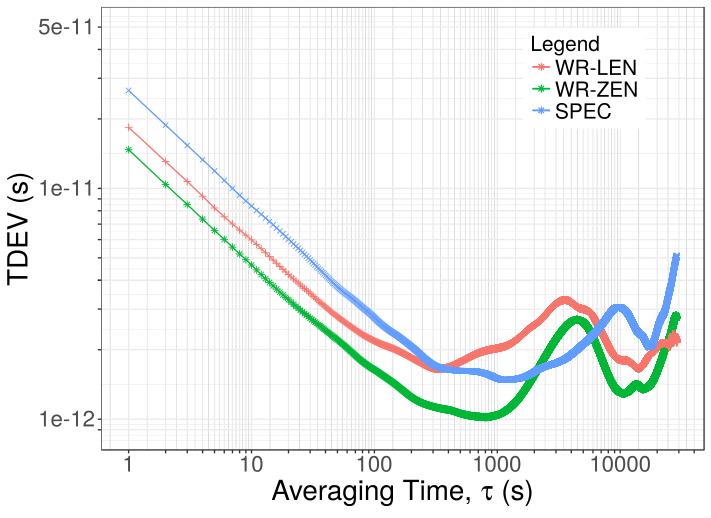
\includegraphics[width=0.7\linewidth]{img/tdev_exp1}
    \caption[TDEV for the WR devices comparison.]{The Time Deviation plot shows 
        that all devices maintain a good PPS performance, nevertheless, the 
        WR-ZEN 
        achieves the best results.}
    \label{fig:tdev_exp1}
\end{figure}
\gutinote{los caption de las figuras tienen que decir lo que es, lo que representa, no nocesariamente evaluar su contenido, para eso ya esta en texto}


Modified Allan Deviation (MDEV) results are included in Figure 
\ref{fig:mdev_exp1}. From the TDEV (\ref{fig:tdev_exp1}) and MDEV (\ref{fig:mdev_exp1}) results we observe that white PM noise dominates from $\tau=1$ to a few hundred  seconds averaging time (depending of the observed device). After that, the rest remains as flicker FM noise.

\begin{figure}
    \centering
    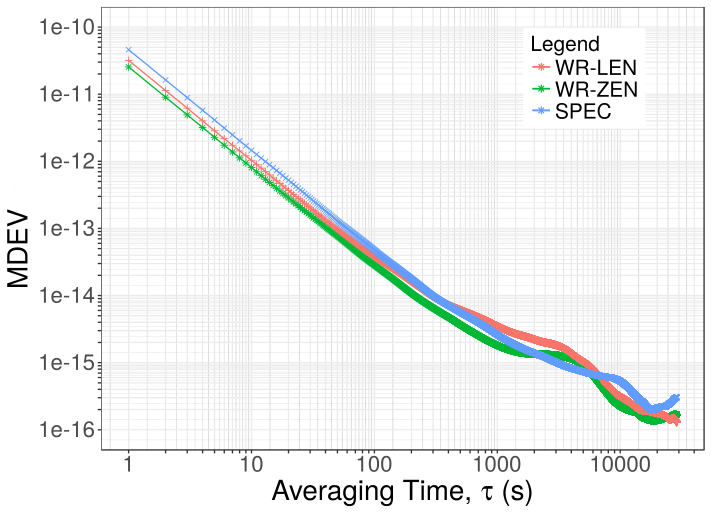
\includegraphics[width=0.7\linewidth]{img/mdev_exp1}
    \caption[MDEV for the WR devices comparison.]{The Modified Allan Deviation 
        plot shows that there is not undesired noise effects on any of the three 
        devices. 
        In the three plots the dominant noise is phase modulated white noise. 
        \textcolor{teal}{usa las siglas}}
    \label{fig:mdev_exp1}
\end{figure}
\gutinote{los caption de las figuras tienen que decir lo que es, lo que representa, no nocesariamente evaluar su contenido, para eso ya esta en texto}


%\begin{table*}\centering
%	\ra{0.8}
%	\begin{tabular}{@{} cccccccccccc@{}}%\toprule
%		& \multicolumn{3}{c}{\bfseries{SPEC}} &&
%		\multicolumn{3}{c}{\bfseries{WR-LEN}} && 
%		\multicolumn{3}{c}{\bfseries{WR-ZEN}} \\
%		\cmidrule(l){2-5}  \cmidrule{6-9} \cmidrule{10-12}
%%		\small{\textbf{$\tau$ (s)} & MDEV & TDEV & MTIE & & MDEV & TDEV & MTIE 	
%%		& & MDEV & TDEV & MTIE} \\
%		\small{\textbf{$\tau$ (s)}} & \tiny{MDEV} & \tiny{TDEV} & 
%		\tiny{MTIE} & & \tiny{MDEV} & \tiny{TDEV} & 
%		\tiny{MTIE} & & \tiny{MDEV} & \tiny{TDEV} & 
%		\tiny{MTIE} \\
%		1 & X & Y & Z && 
%		\bottomrule
%	\end{tabular}
%	\caption{In this table it can be checked out the most relevant statistics 
%	for the device characterization performed in the subsection \ref{subsec: 
%	charact_zen}. \textcolor{red}{esto hay que explicarlo más e intentarlo 
%	meterlo dentro de su sección}}
%	\label{tab:exp1res}
%\end{table*}

Finally, the worst case analysis has been performed with the Maximum Time Interval Error (MTIE) 
statistic (Figure \ref{fig:mtie_exp1}). With the TDEV results, we observed that 
all the WR devices fulfil the 2 ns time budget requirement even for the worst case scenario. 
For the WR-ZEN the difference between the WRS PPS and its PPS is bounded on 1.5e-10 s. Again, the 
WR-ZEN achieves the best results: 3.90e-11 less than the WR-LEN and 1.02e-10 less than the SPEC.

\begin{figure}
	\centering
	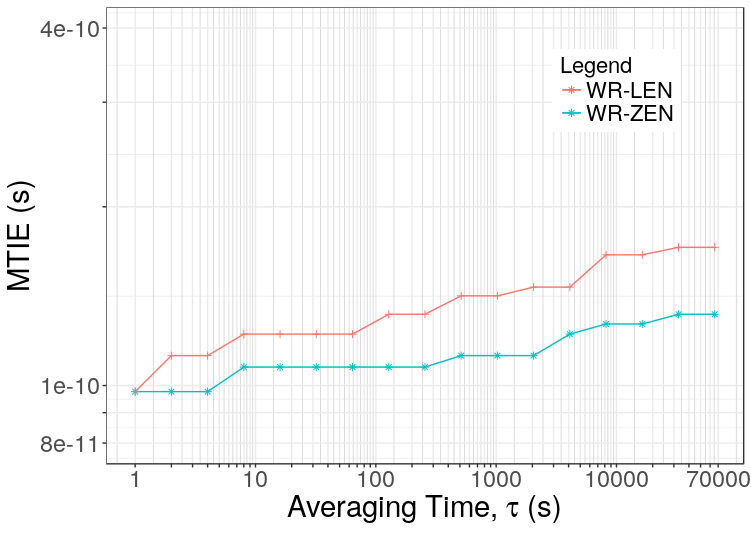
\includegraphics[width=0.7\linewidth]{img/mtie_exp1}
	\caption[MTIE for the WR devices comparison.]{The worst case scenario 
	verifies that the three devices fulfil the time budget requirement. The 
	WR-ZEN with the registered PPS output performs the best of the three.}
	\label{fig:mtie_exp1}
\end{figure}
\gutinote{los caption de las figuras tienen que decir lo que es, lo que representa, no necesariamente evaluar su contenido, para eso ya esta en texto}


The obtained values reveal that the proposed solution fulfils the requirements 
to be used in the SKA telescope's PPS distribution system. Although, it is 
necessary to evaluate it in more realistic conditions before concluding its 
goodness.

\subsection{WR scalability for SKA}
\label{subsec: net_exp}

The next experiment covers a scalability analysis of the WR solution for the 
SKA timing system. In section \ref{sec:ska} we presented an estimation of the final nodes that would be needed to be synchronized for the SKA: around 250 endpoints \textcolor{teal}{se decanta por usar -} that must be synchronized with an accuracy below 2 ns. A WR network with only two hops is suitable to synchronize up to 306 end-nodes by using BC WRSs.

We set up a test network composed of a WRS at the top of the hierarchy, which is locked to an external time reference, another WRS as intermediate BC and a WR-ZEN as an endpoint \textcolor{teal}{se decanta por usar -}. This configuration allows synchronizing up to 306 WR nodes with an expected performance similar to the results obtained in our test for the WR-ZEN.

\begin{figure}
	\centering
	\includegraphics[width=0.7\linewidth]{img/prueba_red}
	\caption[WR Scalability test's setup for SKA]{To evaluate the scalability 
	of the WR solution for the expected SKA timing network, a sample WR 
	network has been evaluated. At the top there is a WRS as GM, a second layer 
	of WRS to finally provide synchronization to the end-nodes (WR-ZEN).}
	\label{fig:pruebared}
\end{figure}

This experiment has been tested under laboratory conditions. A 20 km fibre spool has 
been used to connect each WR device using FiberStore SFPs (SFP-GE-BX80 with 1490/1550 nm wavelengths). 
The PPS phase difference between the WR-ZEN and the WRS in GM mode has been measured  using a Keysight 52320A 
counter for 4 hours.

\begin{figure}
	\centering
	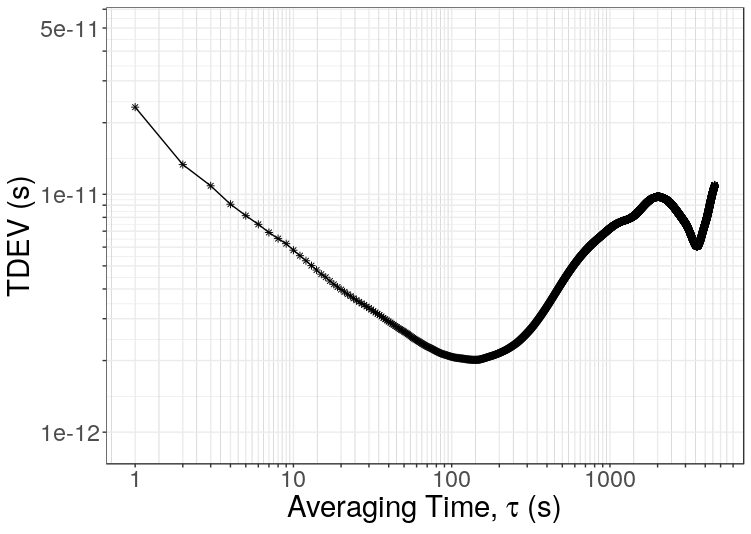
\includegraphics[width=0.7\linewidth]{img/tdev_exp3}
	\caption[TDEV of the end-nodes in the scalability test.]{Time Deviation 
	plot comparing the PPS signal from the end-nodes (WR-ZEN) to the Grand 
	Master of the network.}
	\label{fig:tdevnet}
\end{figure}

TDEV and MTIE values have been calculated by octaves, the numerical 
values can be found in Table \ref{tab:netresults}. For the short-therm 
stability we obtained a TDEV result of 2.32e-11 s. The minimum is reached at 
$\tau=64$, after that, it is observed a frequency drift from $\tau=200$ to 
$\tau=1000$ (see Figure \ref{fig:tdevnet}). The MTIE results show that the maximum 
PPS error, during this test, is bounded below 2e-10 s (see Figure 
\ref{fig:mtienet}).

\begin{table*}\centering
	\ra{0.8}
	\begin{tabular}{@{} rcc@{}}%\toprule
		& TDEV (s)  & MTIE (s) \\ \midrule
		\textbf{$\tau$ (s)}\\
		\small{1}     & 2.32e-11  & 1.36e-10 \\
		%\small{2}     & 1.33315382e-11  & 1.36718750e-10 \\
		%\small{4}     & 9.08699704e-12  & 1.36718750e-10 \\
		\small{8}     & 6.51e-12  & 1.36e-10 \\
		%\small{16}    & 4.48330572e-12  & 1.36718750e-10 \\
		%\small{32}    & 3.22792513e-12  & 1.36718750e-10 \\
		\small{64}    & 2.37e-12  & 1.46e-10 \\
		%\small{128}   & 2.02186966e-12  & 1.46484375e-10 \\
		%\small{256}   & 2.36616321e-12  & 1.46484375e-10 \\
		\small{512}   & 4.38e-12  & 1.61e-10 \\
		\small{1024}  & 7.27e-12  & 1.66e-10 \\
		\small{2048}  & 9.75e-12  & 1.75e-10 \\
		\small{4096}  & 7.97e-12  & 1.90e-10 \\
		%\small{8192}  &                 & 2.00195313e-10 \\
		
		\bottomrule
	\end{tabular}
	\caption{This table contains the Time Deviation and Maximum Time Interval 
	Error results from the scalability test.}
	\label{tab:netresults}
\end{table*}

With those findings, it has been proved that a WR network with two levels can 
provide synchronization to all the equipment expected for the SKA facilities. 
It is also important to mention that some links could be divided into two WR links 
due to the distance between some antennas (e.g. adding a WR device 
between the master WRS and the end-node). Introducing an extra WR level for some 
antennas should not be a problem to fulfil the timing requirements, a prove of 
that can be found in \cite{torres2016scalability}, where the results show that 
even a 10-hop network can reach the required time-budget for SKA.

Although long-distance fibre links have been used for this test, thermal 
influence should be considered before confirming the goodness of the 
WR solution for the SKA's timing distribution system. 

\begin{figure}
	\centering
	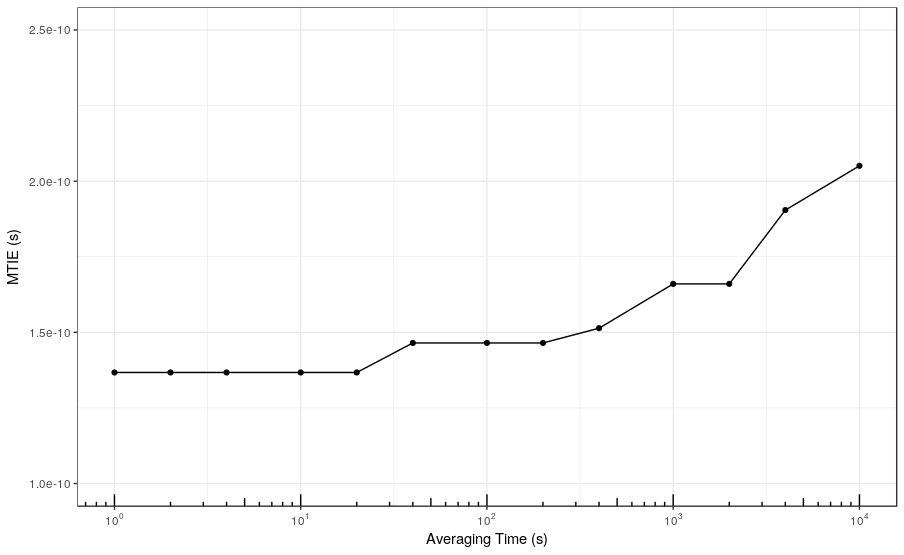
\includegraphics[width=0.7\linewidth]{img/MTIE_exp3}
	\caption[MTIE of the end-nodes in the scalability test.]{Maximum Time 
	Interval Errorplot comparing the PPS signal from the end-nodes (WR-ZEN) to 
	the Grand Master of the network. \textcolor{teal}{cambia esto felipe}}
	\label{fig:mtienet}
\end{figure}
\gutinote{la fuente de esta figura sigue chica. Ponedla como las demas.}

\subsection{Temperature influence on time accuracy}
%\subsection{Fibre operational temperature influence on time accuracy}
\label{subsec:temp}

One of the key aspects of the timing solution for the SKA facilities is the 
evaluation of the influence of the external elements in the timing performance. 
Synchronization signals are spread over hundred of nodes which are connected by 
long distance fibre links. Meteorological elements, such as wind or large 
temperature changes, can alter propagation delays over the fibre 
links. The timing solution must compensate appropriately those effects in order 
to maintain the synchronization performance inside the limits required by the 
SKA's infrastructure. 

The proposed system has been tested by JIVE \cite{jive:website} in the SKA specific dessert zones of 
the South Africa and \cite{paul-boven-paper-icalepcs} describes the main issues 
that must be taken into consideration. The main conclusion of this study is the
need of compensation techniques to control the timing drift because of
temperature changes.

In this contribution, we have focused on the temperature change effect over the 
cable \textit{round-trip} time (CRTT) and the PPS performance. To evaluate this, we have used a climate chamber in the laboratory and some fibre spools of tens of kilometers. Wind impact has not been evaluated due to the lack of the specific equipment in our laboratory. Then, the experiments will only determine temperature effect on synchronization.

Theoretically, WR is able to dynamically calibrate the master-slave 
propagation delay from the total \textit{round-trip} time, and therefore PPS 
offset shall remain constant even when the propagation delay changes. The 
accurate estimation of the one-way propagation delay is achieved by using 
a constant value, $\alpha$, which express the ratio between the propagation time 
with respect to the two wavelengths used in the WR link. Deeper details related to the 
link model can be found at \cite{Wlostowski2011} and \cite{Daniluk2012}.

In the real world, $\alpha$ is temperature dependent, because of the 
refraction index change caused by temperature variations in the fibre.
In laboratory conditions, $\alpha$ is nearly negligible and hence,
the current link model behaves very well for small and mid-distance links. 
It is expected that the WR network planned to be built for SKA will be using long distance
links that can exposed to external elements. 

%In the concrete situation of the South Africa facilities, the chosen location 
% was the Karoo region. This region is a semi-desert area, very adequate to reduce human interferences in the high resolution data acquisition equipment, but with a inconvenient 
%respect to the temperature point of view: desert zones have a high difference 
%between day and night temperatures.

\begin{figure}
	\centering
	\includegraphics[width=0.7\linewidth]{img/tempsetup}
	\caption[Configuration of the climate chamber experiments]{Experimental 
		setup to analyse the influence of the temperature gradient over the 
		fibre link and the synchronization accuracy.}
	\label{fig:tempsetup}
\end{figure}

A series of experiments introducing a 50 km length fibre spool in a climate chamber has been performed.
The CRTT and the master-slave PPS offset have 
been measured for a temperature range from 20\degree C to 50\degree C with 10\degree C steps. 

\begin{table*}\centering
	\ra{0.8}
	\begin{tabular}{@{} cccccc@{}}%\toprule
		& \multicolumn{2}{c}{\bfseries{RTT (ps)}} & &
		\multicolumn{2}{c}{\bfseries{PPS $offset_{SM}$ (ps)}} \\
		\cmidrule(l){2-3}  \cmidrule{5-6}
		\textbf{Spool temp (\degree C)} & $\overline{x}$ & $s$ & & $\overline{x}$ 
		& $s$ \\ \midrule
		\small{20} & 478471695 & 303 & & 193 & 17 \\
		\small{30} & 478503719 & 50  & & 203 & 17 \\
		\small{40} & 478533492 & 807 & & 150 & 17 \\
		\small{50} & 478567050 & 399 & & 110 & 14 \\
		\bottomrule
	\end{tabular}
	\caption{Results of the thermal characterization for an operational fibre 
		temperature in range 20\degree C to 50\degree C with 10\degree C steps.}
	\label{tab:temp}
\end{table*}

Our test is intended to prove the hypothesis that PPS offset is not related to 
the cable \textit{round-trip} time, i.e. changes in CRTT will not affect the 
synchronization accuracy. We have performed a series of experiments where the 
operational temperature of a 50 km fibre link is set in a point from 20\degree C to 
50\degree C. The measurement of the rest of dependent values such as CRTT and PPS offset
was accomplished right after reaching the target temperature.
All the WR equipment was 
calibrated to compensate the characteristic delays of each device 
following the official calibration procedure \cite{man:calib}.  The test setup 
is depicted in figure \ref{fig:tempsetup}.

The most relevant results are included in Table \ref{tab:temp}: (i) the mean 
value of CRTT and PPS offset samples, and (ii) their sample standard deviation. 
A total of 7200 samples (2 hours) per temperature step have been used to 
compute the presented statistics. The amplitude of the CRTT sampled data is 
96496 ps. Dividing it by the temperature range we obtained a CRTT variation of 
3213 ps/C. It is important to remark the huge variation in the propagation delay. 
Considering a synchronization system that is not capable of dynamically 
calibrate that change, the final performance would suffer from an enormous 
degradation, which is unacceptable for the SKA equipment. The peak-to-peak 
difference for the PPS offset is 211 ps which leaves us a 7 ps/C and if we 
divide by the total link length: $0.14 ps/C \cdot km$.

%\begin{figure}
%	\centering
%	\begin{subfigure}[t]{0.48\textwidth}
%		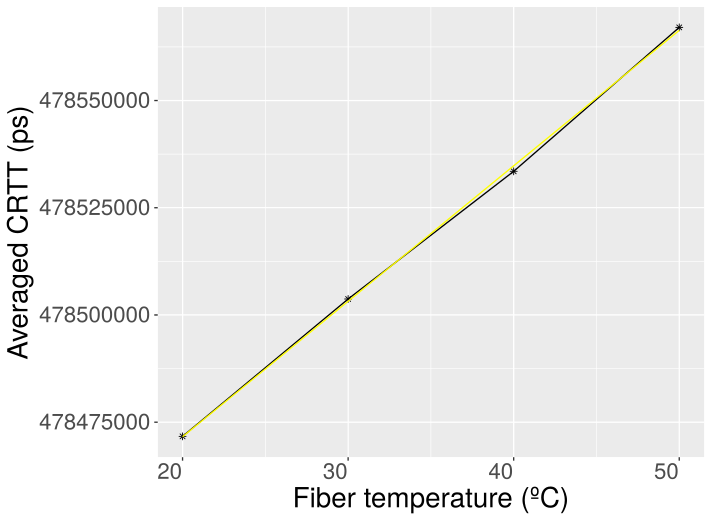
\includegraphics[width=\textwidth]{img/crttvstemp}
%		\caption[CRTT vs. Fiber temperature]{The figure shows the relation 
%			between the fibre temperature and the cable round-trip time.}
%		\label{fig:crttvstemp}
%	\end{subfigure}
%	~ % This symbol adds a white space between images
%	\begin{subfigure}[t]{0.48\textwidth}
%		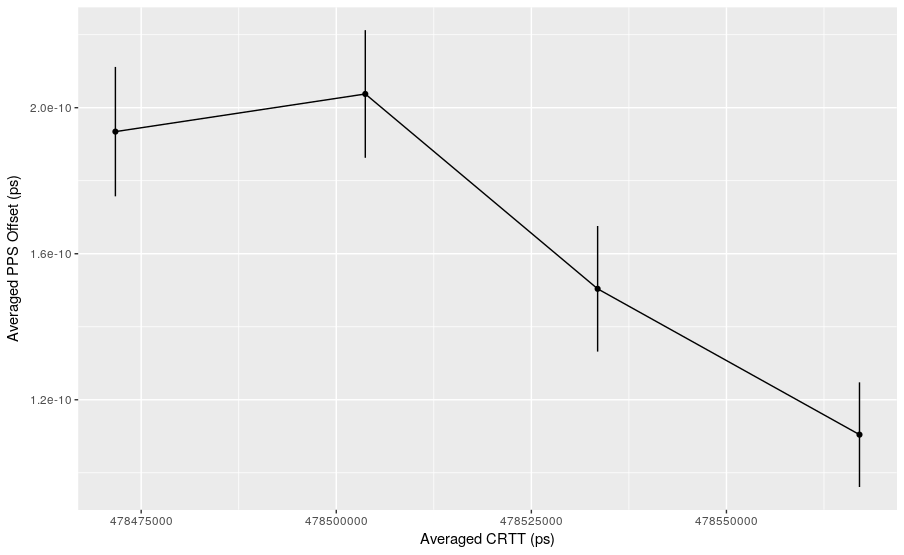
\includegraphics[width=\textwidth]{img/ppsvscrtt}
%		\caption[PPS offset vs. CRTT]{This figure shows how PPS offset is 
%			sightly influenced by changes in the cable round-trip time.}
%		\label{fig:ppsvscrtt}
%	\end{subfigure}
%	\caption{Evaluation of the cable \textit{round-trip} time and the PPS 
%		offset with variable temperature conditions for the fibre link.}
%\end{figure}


	
\begin{figure}[t]
	\centering
	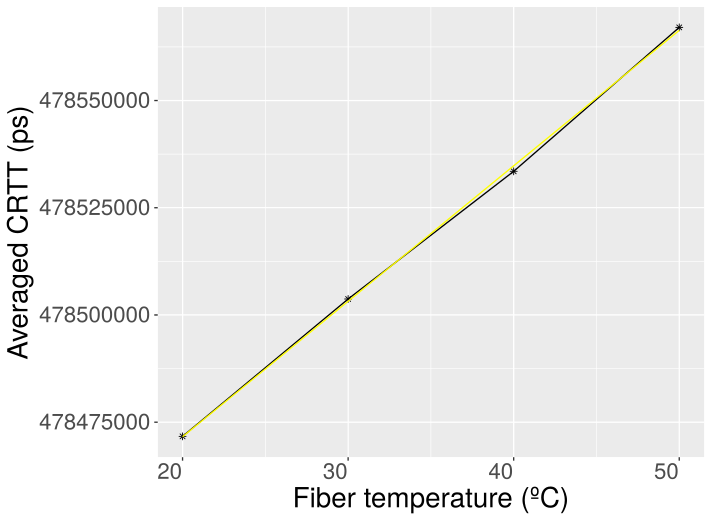
\includegraphics[width=0.7\linewidth]{img/crttvstemp}
	\caption[CRTT vs. Fiber temperature]{The figure shows the relation 
	between the fibre temperature and the cable round-trip time.}
	\label{fig:crttvstemp}
\end{figure}

\begin{figure}[t]
	\centering
	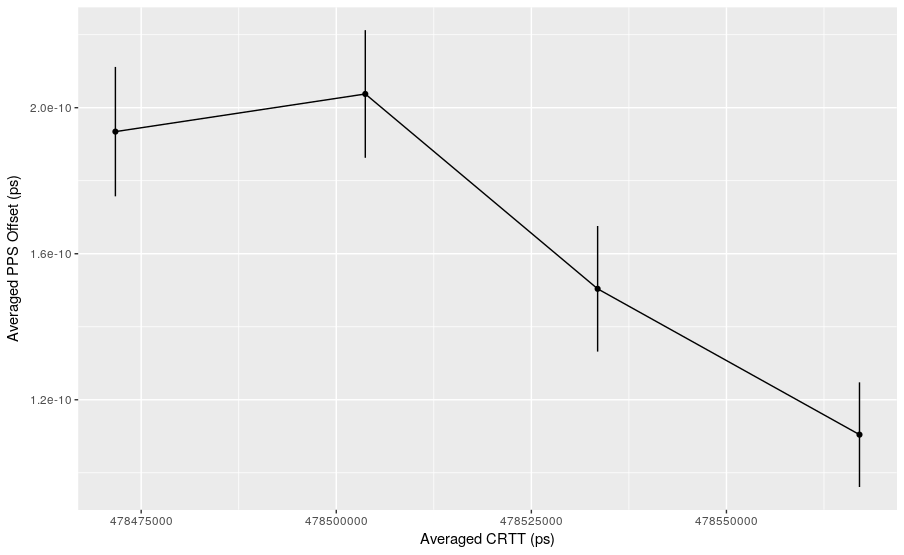
\includegraphics[width=0.7\linewidth]{img/ppsvscrtt}
	\caption[PPS offset vs. CRTT]{This figure shows how PPS offset is 
	sightly influenced by changes in the cable round-trip time.}
	\label{fig:ppsvscrtt}
	\caption{Evaluation of the cable \textit{round-trip} time and the PPS 
	offset with variable temperature conditions for the fibre 
	link.\textcolor{teal}{que ha pasado con esta imagen?}}
\end{figure}

Figure \ref{fig:crttvstemp} shows a clear linear dependency between the 
temperature and the CRTT. Although, the PPS offset is not constant as 
we suppose in our initial hypothesis. The Figure \ref{fig:ppsvscrtt} suggests 
an inverse linear dependency between CRTT and the offset, but if we take the 
standard error values into account, we cannot state clearly that linear 
relation. It must be considered that $\alpha$ is computed experimentally using 
fixed-point arithmetic (the LM32 has no floating-point unit). While it seemed 
to work properly for distances shorter than few km, it may be insufficient 
for such long distances as the ones used in our experiments. Nevertheless, the 
observed offset variation for a long distance link and a 30C temperature 
gradient is only 200 ps. This together with the results from the previous 
experiments make the new PPS distribution system suitable for the SKA 
timing system.